\section{Details on Interpolation and Extrapolation} \label{appendix:methodology}

\subsection{Identifying Treatment Effects}
\label{app:method_identify}

\noindent In the main paper, we discuss three cases of attrition. Below, we elaborate on the methodology we use for each case. \\

\subsubsection{Complete Data}
\label{app:method_fullobs}

\noindent  In the case where we have complete data, we only need to address the compromised randomization
of treatment status in our empirical estimates (see Section~\ref{section:methodsquestions}). Table~\ref{table:nonipw} lists the variables that are fully observed. \\

\noindent Randomization into treatment and control for each cohort occurred after the cohort was split
into two subsamples balanced by gender, maternal IQ,
and number of siblings. Subjects from each subsample were then matched on HRI, and randomized
into their respective experimental groups. Sex, maternal IQ, number of siblings, and HRI
therefore comprise $Z$. To obtain an
unbiased estimate of the treatment effect, we regress the outcome variable on treatment status,
controlling for those four baseline variables and cohort. \\

\noindent We estimate on 1,000 bootstrap resamples of the original ABC/CARE data to estimate sampling uncertainty. We take the mean of the empirical bootstrap distribution as our point estimate, and the standard deviation
of the distribution as the standard error. We estimate these effects on the
whole ABC/CARE sample, as well as the male and female subsamples. This allows us to generate
benefit/cost ratios and rates of return for the pooled sample, male subsample, and female subsample. \\
%Moreover, we are able to obtain more precise estimates of the treatment
%effect for males, as the data for females generally exhibit more noise. See Table \ref{table:nonipw} for the list of outcomes to which we apply this method.

\begin{table}[H]
\begin{threeparttable}
\caption{Variables Estimated without IPW Adjustment}
\label{table:nonipw}
\centering
% CONTENT CREATED ON SPREADSHEET, TREAT AS A .CSV (TAB DELIMITED)
% CAN BE COPIED INTO A SPREADSHEET PROGRAM (EXCEL, LIBRECALC) FOR EDITING
\begin{tabular}{l l}
\toprule
Variable	&	Age	\\
\midrule			
IQ Standard Score	&	2, 3, 4, 5, 6, 7, 8, 12, 15, 21	\\
PIAT Math Standard Score	&	7	\\
Home Total Score	&	0.5, 1.5, 2.5, 3.5, 4.5, 8	\\
Mother Works	&	2, 3, 4, 5	\\
Biological Mother's Education Level	&	2, 3, 4, 5, 9	\\
Father is Home	&	2, 3, 4, 5	\\
Ever Adopted	&		NA \\
Graduated High School	&	NA	\\
Attended Vocation/Tech/Community College	&	NA	\\
Earned Degree from 4-year College	&	NA	\\
Years of Education	&	30	\\
Works a Job	&	30	\\
Total Felony Arrests	&	Mid-30s	\\
Total Misdemeanor Arrests	&	Mid-30s	\\
Total Years Incarcerated	&	30	\\
Self-reported Health	&	30	\\
Number of Cigarettes Smoked Per Day Last Month	&	30	\\
Number of Days Drank Alcohol Last Month	&	30	\\
Number of Days Binge Drank Alcohol Last Month	&	30	\\
Program Costs	&	0--26	\\
Control Contamination Costs	&	0--26	\\
Education Costs	&	0--26	\\
Medical Expenditure &	8--30	\\
Justice System Costs	&	0--50	\\
Prison Costs	&	0--50	\\
Victimization Costs	&	0--50	\\
\bottomrule			
\end{tabular}
\begin{tablenotes}
\footnotesize
\item Note: The table above lists the variables for which we do not apply IPW when estimating
treatment effects.
\end{tablenotes}
\end{threeparttable}
\end{table}


\subsubsection{Partially Complete Data}
\label{app:method_partialobs}

\noindent Given the small sample size of the ABC/CARE data, we consider outcome variables with fewer than 100 observations
as having a sizable rate of attrition. These variables include parental income at ages 2, 3, 4, 5, 9, 12,
and 15, for which we observe no more than 91 subjects at any given age; and the health survey at
age 34, for which we observe no more than 72 subjects. \\

\noindent We weight each subject by
his/her propensity to select into treatment and propensity to respond. We estimate the
former with a logit model for treatment status, controlling for baseline
variables used to determine randomization into treatment status: cohort,
maternal IQ, number of siblings, HRI, and sex (in the case of pooled estimates). \\

\noindent To estimate the propensity to respond, we estimate a logit model of observing the outcome,
controlling for treatment status and three additional covariates. The additional covariates are
chosen amongst a set of variables likely to be correlated with non-response rates for the outcome variable.
This set of variables includes baseline characteristics determining randomization,
baseline variables other than randomization, and observed adult outcomes potentially affected by
treatment. To select these variables, we estimate the
aforementioned logit model controlling for treatment status and every three-variable combination from
the described set of variables. The model with the lowest Akaike Information Criteria (AIC) value is used to estimate the propensity
to respond. We limit the number of covariates in our logit models to three as this noticeably reduces the frequency of bootstrap resamples which exhibit perfect separation in the covariates. \\

\noindent To estimate the treatment effect, we regress the outcome of interest on treatment status, and weight the
observations by the inverse of the product of the two estimated propensity scores. This procedure is performed on 1,000 bootstrap resamples of the original ABC/CARE data.
We take the mean of the empirical bootstrap distribution as our point estimate, and the standard deviation
of the distribution as the standard error. We carry out this procedure for the
pooled sample, male subsample, and female subsample. Table~\ref{table:ms_attrit_pooled} through Table~\ref{table:ms_attrit_males} summarize the model selection for IPW adjustment for each partially observed outcome. \\

\paragraph{Parental Income}

\noindent Parental income is reported at ages 0, 2, 3, 4, 5, 9, 12, and 15, allowing us to directly estimate
the treatment effect on parental income at those ages. Given the rate of attrition in
parental income from age 2 onwards, we estimate these treatment effects accounting for attrition
with IPW weights.
To obtain a more complete picture of how the
program affected parental income, we estimate the treatment effect in the missing ages by linearly
interpolating the treatment effects between the years for which we observe parental income. We assume
there are no impacts from age 16 onwards (i.e. a treatment effect of 0). \textbf{[JJH: Jorge, can we not do better? Impute profiles using PSID?]}\textbf{[JLG: the reason for doing a linear interpolation is that the support in the PSID doesn't let us do much here. The information on the parents is not very complete. PSID of course surveys parents and children, but the matches here are adults and their parents barely appear in PSID. In other words, we are matching the ABC/CARE subjects to individuals who are not young enough as for us to obtain a good income profile of their parents.  We have eight observations between ages 0 and 15 and we are relying on that now.]} \\

\begin{sidewaystable}[H]
\caption{Model Selection for Attrition IPW \\ Pooled }
\label{table:ms_attrit_pooled}
\centering
\begin{adjustbox}{max width=\textwidth}
\begin{threeparttable}
% CONTENT CREATED ON SPREADSHEET, TREAT AS A .CSV (TAB DELIMITED)
% CAN BE COPIED INTO A SPREADSHEET PROGRAM (EXCEL, LIBRECALC) FOR EDITING
\scriptsize
\begin{tabular}{l r r l l l}
\toprule											
Partially Observed Outcomes	&	Age	&	N	&	\multicolumn{3}{c}{Variables Used to Produce IPW}	\\
\midrule	
IQ Score 				& 6.5 	& 126   & High Risk Index (HRI)	& APGAR 1 min.	&  Cohort \\
IQ Score 				& 7 	& 118   & High Risk Index (HRI)	& APGAR 5 min.	&  Cohort \\
IQ Score 				& 8 	& 125   & High Risk Index (HRI)	& APGAR 1 min.	&  Cohort \\
\\										
Achievement Score 		& 5.5	& 105 	& High Risk Index (HRI)	& APGAR 1 min.	&  Cohort \\ 
Achievement Score 		& 6		& 124 	& High Risk Index (HRI)	& APGAR 1 min.	&  Cohort \\ 
Achievement Score 		& 6.5	& 89 	& High Risk Index (HRI)	& APGAR 1 min.	&  Cohort \\ 
Achievement Score 		& 7		& 90 	& High Risk Index (HRI)	& APGAR 1 min.	&  Cohort \\ 
Achievement Score 		& 7.5	& 121 	& High Risk Index (HRI)	& APGAR 1 min.	&  Cohort \\ 
Achievement Score 		& 8		& 123 	& High Risk Index (HRI)	& APGAR 1 min.	&  Cohort \\ 
Achievement Score 		& 8.5	& 122 	& High Risk Index (HRI)	& APGAR 5 min.	&  Cohort \\ 
\\
Parental Labor Income	&	1.5	&	112	& Mother's Age at Baseline	& APGAR 1 min.	&  Cohort \\
 Parental Labor Income	&	2.5	&	112	&	Mother's Age at Baseline	& APGAR 1 min.	&  Cohort \\
 Parental Labor Income	&	3.5	&	110	&	Mother's Age at Baseline	& APGAR 1 min.	&  Cohort \\
 Parental Labor Income	&	8	&	87	&	High Risk Index (HRI)	& APGAR 1 min.	&  Cohort \\
 Parental Labor Income	&	12	&	108	&	High Risk Index (HRI)	& APGAR 1 min.	&  Cohort \\
 Parental Labor Income	&	15	&	92	&	APGAR 5 min. & 	Premature at Birth & Number of Siblings, Baseline \\
 Parental Labor Income	&	21	&	73	&	High Risk Index (HRI)	& APGAR 1 min.	&  Cohort \\
\\
HOME Score				& 8		& 	100 & 	High Risk Index (HRI)	& APGAR 1 min.	&  Cohort \\
\\
Father at Home			& 8		& 	116 & 	High Risk Index (HRI)	& APGAR 1 min.	&  Cohort \\
\\
Subject Public Transfer Income	&	21	&	105	& High Risk Index (HRI) & APGAR 1 min. & Cohort \\
 \\
Total Felony Arrests		& Mid-30s	& 115 &	APGAR 1 min. & APGAR 5 min. & Cohort	\\
Total Misdemeanor Arrests	& Mid-30s	& 115 &	APGAR 1 min. & APGAR 5 min. & Cohort	\\
 \\
 Self-reported Health	&	Mid-30s	&	92	&	APGAR 1 min. & APGAR 5 min. & Premature at Birth	\\
 Self-reported Drug User	&	Mid-30s	&	89	&	APGAR 1 min. & APGAR 5 min. & Premature at Birth	\\
 Systolic Blood Pressure (mm Hg)	&	Mid-30s	&	90	&	APGAR 1 min. & Premature at Birth & Number of Siblings, Baseline	\\
 Diastolic Blood Pressure (mm Hg)	&	Mid-30s	 &	90	&	APGAR 1 min. & Premature at Birth & Number of Siblings, Baseline	\\
 Prehypertension, Sys. B.P. $>$ 120 or Dys. B.P. $>$ 80	&	Mid-30s	&	90	&	APGAR 1 min. & Premature at Birth & Number of Siblings, Baseline	\\
 Hypertension, Sys. B.P. $>$ 140 or Dys. B.P. $>$ 90	&	Mid-30s	&	90	&	APGAR 1 min. & Premature at Birth & Number of Siblings, Baseline	\\
 High-Density Lipoprotein (HDL) Cholesterol (mg/dL)	&	Mid-30s	&	93	&	APGAR 1 min. & Premature at Birth & Number of Siblings, Baseline	\\
 Dyslipidemia (HDL $<$ 40 mg/dL)	&	Mid-30s	&	93	&	APGAR 1 min. & Premature at Birth & Number of Siblings, Baseline	\\
 Hemoglobin Level (\%)	&	Mid-30s	&	92	&	APGAR 1 min. & Premature at Birth & Number of Siblings, Baseline	\\
 Prediabetes, Hemoglobin $>$ 5.7\%	&	Mid-30s	&	92	&	APGAR 1 min. & Premature at Birth & Number of Siblings, Baseline	\\
 Diabetes, Hemoglobin $>$ 6.5\%	&	Mid-30s	&	92	&	APGAR 1 min. & Premature at Birth & Number of Siblings, Baseline	\\
 Vitamin D Deficiency ($<$ 20 ng/mL)	&	Mid-30s	&	93	&	APGAR 1 min. & Premature at Birth & Number of Siblings, Baseline	\\
 Measured BMI	&	Mid-30s	&	88	&	APGAR 1 min. & APGAR 5 min. & Premature at Birth \\
 Obesity (BMI $>$ 30)	&	Mid-30s	&	90	&	APGAR 1 min. & APGAR 5 min. & Premature at Birth \\
 Severe Obesity (BMI $>$ 35)	&	Mid-30s	&	91	&	APGAR 1 min. & APGAR 5 min. & Premature at Birth \\
 Waist-hip Ratio	&	Mid-30s	&	84	& APGAR 1 min. & Premature at Birth & Number of Siblings, Baseline \\
 Abdominal Obesity	&	Mid-30s	&	84	& APGAR 1 min. & Premature at Birth & Number of Siblings, Baseline \\
 Framingham Risk Score	&	Mid-30s	&	88	& APGAR 1 min. & Premature at Birth & Number of Siblings, Baseline \\
 Brief Symptom Survey (BSI) Score & Mid-30s & 92 &	APGAR 1 min. & APGAR 5 min. & Premature at Birth	\\
\bottomrule											
\end{tabular}
\begin{tablenotes}
\tiny
\item Note: The table above lists the variables used to generate the
inverse probability weights we use to account for attrition. We estimate a logit model for observing the outcome variable,
controlling for treatment, and three additional covariates depending on the outcome
variable. The additional variables are chosen from a list of covariates possibly affecting
response rates. The set yielding the lowest Akaike Information Criteria value is used to
generate the IPW weights, and are listed in the table above.
\end{tablenotes}
\end{threeparttable}
\end{adjustbox}
\end{sidewaystable}

\begin{sidewaystable}[H]
\caption{Model Selection for Attrition IPW \\ Females }
\label{table:ms_attrit_females}
\centering
\begin{adjustbox}{max width=\textwidth}
\begin{threeparttable}
% CONTENT CREATED ON SPREADSHEET, TREAT AS A .CSV (TAB DELIMITED)
% CAN BE COPIED INTO A SPREADSHEET PROGRAM (EXCEL, LIBRECALC) FOR EDITING
\tiny
\begin{tabular}{l r r l l l}
\toprule										
Variable	&	Age	&	Obs.	&	(1)	&	(2)	&	(3)	\\
\midrule											
Parental Labor Income	&	2	&	33	&	Subject Birth Year	&	Mother Works, age 5	&	Father works before pregnancy	\\
Parental Labor Income	&	3	&	33	&	Subject Birth Year	&	Mother Works, age 5	&	Father works before pregnancy	\\
Parental Labor Income	&	4	&	31	&	Subject Birth Year	&	Father works before pregnancy	&	Siblings in Household, age 5	\\
Parental Labor Income	&	5	&	44	&	Mother Works before Pregnant	&	Mother Works, age 5	&	Father works before pregnancy	\\
Parental Labor Income	&	9	&	40	&	Mother Works, age 5	&	HRI 2: No Maternal Relatives	&	Father works before pregnancy	\\
Parental Labor Income	&	12	&	45	&	Subject Birth Year	&	Mother Works, age 5	&	Father works before pregnancy	\\
Parental Labor Income	&	15	&	47	&	Mother Works, age 5	&	HRI 2: No Maternal Relatives	&	Father works before pregnancy	\\
\\
Subject Labor Income	&	21	&	51	&	Mother's WAIS Performance IQ	&	Mother's Age at entry	&	ASR t-score: Attention Deficit and Hyperactivity	\\
Subject Labor Income	&	30	&	53	&	HRI 10: Other special circumstances	&	ASR t-score: Substance Abuse	&	Years of Education	\\
Subject Public Transfer Income	&	21	&	49	&	Mother's WAIS Comprehension	&	Number of cigarettes smoked per day	&	ASR t-score: Attention Deficit and Hyperactivity	\\
Subject Public Transfer Income	&	30	&	53	&	HRI 10: Other special circumstances	&	ASR t-score: Substance Abuse	&	Years of Education	\\
\\
Self-reported Health	&	Mid-30s	&	40	&	Length at birth	&	ASR t-score: Substance Abuse	&	Years of Education	\\
Self-reported Drug User	&	Mid-30s	&	40	&	Length at birth	&	ASR t-score: Substance Abuse	&	Years of Education	\\
Systolic Blood Pressure (mm Hg)	&	Mid-30s	&	40	&	Length at birth	&	ASR t-score: Substance Abuse	&	Years of Education	\\
Diastolic Blood Pressure (mm Hg)	&	Mid-30s	&	40	&	Length at birth	&	ASR t-score: Substance Abuse	&	Years of Education	\\
Prehypertension, Sys. B.P. $>$ 120 or Dys. B.P. $>$ 80	&	Mid-30s	&	40	&	Length at birth	&	ASR t-score: Substance Abuse	&	Years of Education	\\
Hypertension, Sys. B.P. $>$ 140 or Dys. B.P. $>$ 90	&	Mid-30s	&	40	&	Length at birth	&	ASR t-score: Substance Abuse	&	Years of Education	\\
High-Density Lipoprotein (HDL) Cholesterol (mg/dL)	&	Mid-30s	&	40	&	Length at birth	&	ASR t-score: Substance Abuse	&	Years of Education	\\
Dyslipidemia (HDL $<$ 40 mg/dL)	&	Mid-30s	&	40	&	Length at birth	&	ASR t-score: Substance Abuse	&	Years of Education	\\
Hemoglobin Level (\%)	&	Mid-30s	&	39	&	Length at birth	&	ASR t-score: Substance Abuse	&	Years of Education	\\
Prediabetes, Hemoglobin $>$ 5.7\%	&	Mid-30s	&	39	&	Length at birth	&	ASR t-score: Substance Abuse	&	Years of Education	\\
Diabetes, Hemoglobin $>$ 6.5\%	&	Mid-30s	&	39	&	Length at birth	&	ASR t-score: Substance Abuse	&	Years of Education	\\
Vitamin D Deficiency ($<$ 20 ng/mL)	&	Mid-30s	&	40	&	Length at birth	&	ASR t-score: Substance Abuse	&	Years of Education	\\
Measured BMI	&	Mid-30s	&	40	&	Length at birth	&	ASR t-score: Substance Abuse	&	Years of Education	\\
Obesity (BMI $>$ 30)	&	Mid-30s	&	40	&	Length at birth	&	ASR t-score: Substance Abuse	&	Years of Education	\\
Severe Obesity (BMI $>$ 35)	&	Mid-30s	&	40	&	Length at birth	&	ASR t-score: Substance Abuse	&	Years of Education	\\
Waist-hip Ratio	&	Mid-30s	&	37	&	Length at birth	&	ASR t-score: Substance Abuse	&	Years of Education	\\
Abdominal Obesity	&	Mid-30s	&	37	&	Length at birth	&	ASR t-score: Substance Abuse	&	Years of Education	\\
Framingham Risk Score	&	Mid-30s	&	39	&	Length at birth	&	ASR t-score: Substance Abuse	&	Years of Education	\\
\bottomrule																																	
\end{tabular}
\begin{tablenotes}
\tiny
\item Note: The table above lists the variables used to generate the
inverse probability weights we use to account for attrition. We estimate a logit model for observing the outcome variable,
controlling for treatment, and three additional covariates depending on the outcome
variable. The additional variables are chosen from a list of covariates possibly affecting
response rates. The set yielding the lowest Akaike Information Criteria value is used to
generate the IPW weights, and are listed in the table above.
\end{tablenotes}
\end{threeparttable}
\end{adjustbox}
\end{sidewaystable}



\begin{sidewaystable}[H]
\caption{Model Selection for Attrition IPW \\ Males }
\label{table:ms_attrit_males}
\centering
\begin{adjustbox}{max width=\textwidth}
\begin{threeparttable}
% CONTENT CREATED ON SPREADSHEET, TREAT AS A .CSV (TAB DELIMITED)
% CAN BE COPIED INTO A SPREADSHEET PROGRAM (EXCEL, LIBRECALC) FOR EDITING
\tiny
\begin{tabular}{l r r l l l}
\hline\hline											
Variable	&	Age	&	Obs.	&	(1)	&	(2)	&	(3)	\\
\hline											
Parent Labor Income	&	2	&	39	&	Subject Birth Year	&	Mother Works, age 3	&	Siblings in Household, age 3	\\
Parent Labor Income	&	3	&	39	&	Subject Birth Year	&	Mother Works, age 3	&	Father works before pregnancy	\\
Parent Labor Income	&	4	&	38	&	Subject Birth Year	&	Mother Works, age 4	&	Siblings in Household, age 3	\\
Parent Labor Income	&	5	&	42	&	Mother Works, age 3	&	Mother Works, age 4	&	Siblings in Household, age 5	\\
Parent Labor Income	&	9	&	42	&	Mother Works, age 3	&	Father home, age 5	&	Siblings in Household, age 5	\\
Parent Labor Income	&	12	&	46	&	Subject Birth Year	&	Mother Works, age 4	&	Father home, age 5	\\
Parent Labor Income	&	15	&	43	&	Mother Works, age 4	&	Father works before pregnancy	&	Siblings in Household, age 5	\\
\\
Subject Labor Income	&	21	&	45	&	HRI 10: Other special circumstances	&	Gestational Age $\leq$ 36	&	ASR t-score: Substance Abuse	\\
Subject Labor Income	&	30	&	47	&	Father's Age at entry	&	Mother Married at entry	&	ASR t-score: Substance Abuse	\\
Subject Public Transfer Income	&	21	&	48	&	Father's Age at entry	&	Gestational Age $\leq$ 36	&	Years of Education	\\
Subject Public Transfer Income	&	30	&	48	&	Mother's WAIS Performance IQ	&	ASR t-score: Antisocial Personality Problems	&	Had physical exam for illness in last 2 years	\\
\\
Self-reported Health	&	Mid-30s	&	30	&	HRI 2: No Maternal Relatives	&	ASR t-score: Substance Abuse	&	ASR t-score: Antisocial Personality Problems	\\
Self-reported Drug User	&	Mid-30s	&	27	&	Gestational Age $\leq$ 36	&	ASR t-score: Substance Abuse	&	Had physical exam for illness in last 2 years	\\
Systolic Blood Pressure (mm Hg)	&	Mid-30s	&	28	&	Gestational Age $\leq$ 36	&	ASR t-score: Substance Abuse	&	Had physical exam for illness in last 2 years	\\
Diastolic Blood Pressure (mm Hg)	&	Mid-30s	&	28	&	Gestational Age $\leq$ 36	&	ASR t-score: Substance Abuse	&	Had physical exam for illness in last 2 years	\\
Prehypertension, Sys. B.P. $>$ 120 or Dys. B.P. $>$ 80	&	Mid-30s	&	28	&	Gestational Age $\leq$ 36	&	ASR t-score: Substance Abuse	&	Had physical exam for illness in last 2 years	\\
Hypertension, Sys. B.P. $>$ 140 or Dys. B.P. $>$ 90	&	Mid-30s	&	28	&	Gestational Age $\leq$ 36	&	ASR t-score: Substance Abuse	&	Had physical exam for illness in last 2 years	\\
High-Density Lipoprotein (HDL) Cholesterol (mg/dL)	&	Mid-30s	&	31	&	Gestational Age $\leq$ 36	&	ASR t-score: Substance Abuse	&	Had physical exam for illness in last 2 years	\\
Dyslipidemia (HDL $<$ 40 mg/dL)	&	Mid-30s	&	31	&	Gestational Age $\leq$ 36	&	ASR t-score: Substance Abuse	&	Had physical exam for illness in last 2 years	\\
Hemoglobin Level (\%)	&	Mid-30s	&	31	&	Gestational Age $\leq$ 36	&	ASR t-score: Substance Abuse	&	Had physical exam for illness in last 2 years	\\
Prediabetes, Hemoglobin $>$ 5.7\%	&	Mid-30s	&	31	&	Gestational Age $\leq$ 36	&	ASR t-score: Substance Abuse	&	Had physical exam for illness in last 2 years	\\
Diabetes, Hemoglobin $>$ 6.5\%	&	Mid-30s	&	31	&	Gestational Age $\leq$ 36	&	ASR t-score: Substance Abuse	&	Had physical exam for illness in last 2 years	\\
Vitamin D Deficiency ($<$ 20 ng/mL)	&	Mid-30s	&	31	&	Gestational Age $\leq$ 36	&	ASR t-score: Substance Abuse	&	Had physical exam for illness in last 2 years	\\
Measured BMI	&	Mid-30s	&	26	&	Gestational Age $\leq$ 36	&	ASR t-score: Substance Abuse	&	Had physical exam for illness in last 2 years	\\
Obesity (BMI $>$ 30)	&	Mid-30s	&	28	&	Father works before pregnancy	&	ASR t-score: Substance Abuse	&	ASR t-score: Attention Deficit and Hyperactivity	\\
Severe Obesity (BMI $>$ 35)	&	Mid-30s	&	29	&	HRI 2: No Maternal Relatives	&	Mother's WAIS Comprehension	&	Number of times smoked marijuana	\\
Waist-hip Ratio	&	Mid-30s	&	25	&	Gestational Age $\leq$ 36	&	ASR t-score: Substance Abuse	&	Had physical exam for illness in last 2 years	\\
Abdominal Obesity	&	Mid-30s	&	25	&	Gestational Age $\leq$ 36	&	ASR t-score: Substance Abuse	&	Had physical exam for illness in last 2 years	\\
Framingham Risk Score	&	Mid-30s	&	27	&	Gestational Age $\leq$ 36	&	ASR t-score: Substance Abuse	&	Had physical exam for illness in last 2 years	\\
\hline\hline																							
\end{tabular}
\begin{tablenotes}
\tiny
\item Note: The table above lists the variables used to generate the
inverse probability weights we use to account for attrition. We estimate a logit model for observing the outcome variable,
controlling for treatment, and three additional covariates depending on the outcome
variable. The additional variables are chosen from a list of covariates possibly affecting
response rates. The set yielding the lowest Akaike Information Criteria value is used to
generate the IPW weights, and are listed in the table above.
\end{tablenotes}
\end{threeparttable}
\end{adjustbox}
\end{sidewaystable}


\subsubsection{Incomplete Data}
\label{app:method_noobs}

\paragraph{Subject Income}

\noindent Labor and public-transfer income of subjects are only observed at ages 21 and 30.\footnote{At age 21, public-transfer income includes Aid to
Families with Dependent Children (AFDC) subsidies, food stamps, survivor benefits, disability
benefits, social security, rent subsidies, and fuel subsidies. At age 30, public-transfer income includes food stamps, welfare, housing assistance, workman's
compensation, disability, social security, supplemental security income, unemployment benefits,
worker's compensation insurance, fuel subsidies, educational and aid grants, and other forms of welfare.} In order to obtain a complete measure of the impact of the ABC/CARE programs on subject income, we interpolate the income streams of subjects for ages 22 to 29, and extrapolate income streams for ages 31 to 67 using three auxiliary datasets described below: NLSY, CNLSY, and PSID. \\

\noindent \textbf{The National Longitudinal Survey of Youth (NLSY)} is a longitudinal survey beginning in 1979 that follows individuals born between 1957 and 1964. The initial interview included 12,686 respondents aged 14 to 22. The survey was designed to include 6,111 individuals representing the non-institutionalized civilian population, a supplemental sample of 5,295 civilian Hispanics, Latinos, blacks, non-blacks/non-Hispanics, and economically disadvantaged youth, and a sample of 1,280 who served in the military as of September 30, 1978. When appropriately weighted, the NLSY is nationally representative of the youth living in the U.S. on January 1, 1979. We include individuals from all three subsamples in our analysis. \\

\noindent The NLSY collected data on labor market participation, education, family background, family life, health issues, assets and income, government program participation, and measures of cognitive skills. We use these data to estimate a prediction model for subject income for ages 31 through 67. \\

\noindent We restrict the NLSY sample to individuals with labor income less than \$300,000 (2014 USD) at any given year. With the mean labor income (2014 USD) in the ABC sample being \$12,232 at age 21 and \$32,782 at age 30, and the maximum reported being \$189,938, the cut-off we impose on the auxiliary data is high enough so that everyone in the ABC/CARE sample is represented, yet low enough to exclude high-earning individuals in the auxiliary sample that do not reflect the ABC/CARE sample well. \\

\noindent We do not impose a restriction on birth year on the NLSY as all respondents are aged between 47 and 55 at the time of the last interview (conducted in 2012). This age range is within the 31--67 range for which we extrapolate the income of the ABC/CARE subjects. \\

\noindent Given the biennial nature of the NLSY, we only observe each subject at either odd or even ages. Not only does this reduce the size of the sample on which we fit our prediction model at each age, but it can introduce biases associated with the odd-aged and even-aged cohorts. To address this issue, we perform a linear interpolation on the variables in the NLSY data that enter into our prediction model. This allows us to estimate our prediction model on all subjects of the NLSY satisfying our restrictions at every age. \\

\noindent \textbf{The Children of the National Longitudinal Survey of Youth (CNLSY)} is a survey of the children of the mothers from the NLSY, beginning in 1986. At the time of the initial interview, the ages of the children surveyed ranged from 0 to 23. As of 2010, the CNLSY sample includes 11,504 children born to NLSY mothers. With appropriate weights, the CNLSY may be considered nationally representative of children born to women who were aged 14 to 22 during 1979. Interviews were conducted annually between 1986 and 1994, and biennially thereafter. \\

\noindent Similar to the NLSY, the CNLSY collected data on cognitive ability, motor and social development, home environment, health information, education, attitudes, employment, income, family decisions, and more. We use these data to estimate a prediction model for subject income for ages 22 through 29. \\

\noindent As we did with the NLSY, we restrict the CNLSY sample to individuals with labor income less than \$300,000 (2014 USD) at any given year. In addition to this, we limit the sample to subjects born between 1978 and 1983. Because the CNLSY data extend to 2012, this implies that we use the most recent data from the CNLSY in which individuals are aged 29 to 34. Finally, given the biennial nature of the survey, we perform a linear interpolation on the variables that enter into our prediction model. This allows us to use as much of the CNLSY data as possible at every age when interpolating subject income. \\

\noindent \textbf{The Panel Survey of Income Dynamics (PSID)} is a longitudinal household survey containing between 5,000 and 8,500 families in each wave. It began as a yearly survey in 1968 and has been fielded biennially since 1996. When appropriately weighted, the PSID is designed to be representative of U.S. households. The PSID provides extensive information concerning demographics, economic outcomes, health outcomes, marriage and fertility, and more. In addition to using the PSID to forecast future earnings of ABC/CARE subjects, we use the PSID to forecast health outcomes. See Appendix \ref{section:data_psid} for details on how the PSID relates to health outcomes. \\

\noindent Similar to the CNLSY, we restrict the PSID to individuals born between 1945 and 1981. Because the data extend to 2013, we use the most recent subsample of individuals aged 30 to 67. We also exclude all individuals with labor income exceeding \$300,000 (2014 USD) in any given year. Finally, given the biennial nature of the survey, we perform a linear interpolation on the variables that enter into our prediction model. This allows us to use as much of the PSID data as possible at every age to interpolate subject income. \\

\noindent We assume common support between these auxiliary datasets and the analysis sample. This is required in order for us to reliably use external data to provide inference for the ABC/CARE samples. Figure~\ref{fig:support} validates this assumption by displaying the overlapping support sets of ABC/CARE and our auxiliary data for the variables used to interpolate and extrapolate earnings.  \\

\noindent \textbf{[JJH: Jorge, these are hard to read and we are missing many of the variables we use to project.]} \\
\textbf{[JLG: We are assuming common support in two vector of variables: W (pre-program variables) and X (programs possibly affected by treatment). In our empirical application we let:} \\

\noindent $\mathbf{W =}$ \textbf{male indicator, black indicator, mother's education} \\
\noindent $\mathbf{X =} $ \textbf{PIAT scores at ages 5-7, years of education at age 30 income at ages 21 and 30, BMI at age 34}


\begin{enumerate}
\item \textbf{For all of the variables in W,X except for the male and black indicators, you can find a plot showing the overlap in the support between the experimental and the auxiliary samples.} 

\item \textbf{There is a real full overlap in the sense that the support in the auxiliary samples completely contains the support in the experimental sample.} 

\item \textbf{I can print this in color for you tomorrow, but if you have a screen handy, there is no doubt of the overlap.} 

\item \textbf{The reasons why additional samples were brought up was (a) timing of the variables; (b) common support itself. Here is an example. For labor income at age 21, the cNLSY provided us the widest support given the age of its individuals. It was not necessary to bring in more samples. For labor income at age 30, we did need to bring in more samples because the support in cNLSY was not covering the support in the experimental data. This is why you see different auxiliary samples change across plots.}

\item \textbf{For the male indicator we do not have a common support issue. For the black indicator we don't either, but you might want to ask why we do not keep only blacks to perform the interpolations and extrapolations. The answer is: we did try an exercise in which we only kept the black sample. The common support conditions struggle a little more to be satisfied but we went all the way to compute the CBA using the black sample only. The standard errors grow but not to a great extent. I wouldn't worry about someone asking us to perform that exercise but I think it's better to keep the full sample. At the end of the day, a lot of the other variables we are using predict well the disadvantage of the sample.} 

\item  \textbf{How do we choose the variables in W,X and why we didn't choose others? This is basically a restriction imposed by the availability of the the data in the experimental and non-experimental sources. We did a careful cross-walk and maximized the amount of variables we were able to use.} 
\end{enumerate}
\textbf{These points are the reasons why you see these plots and no more in this appendix.]} \\

\noindent \textbf{[JLG: plots were remade and these pages were printed in color for you.]}


\begin{figure}[H]
	\caption{Support of ABC/CARE and Auxiliary Data} \label{fig:support}
	\begin{subfigure}[h]{0.9\textwidth}
	\centering
	\caption{Income at Age 21} \label{fig:support_inc21}
	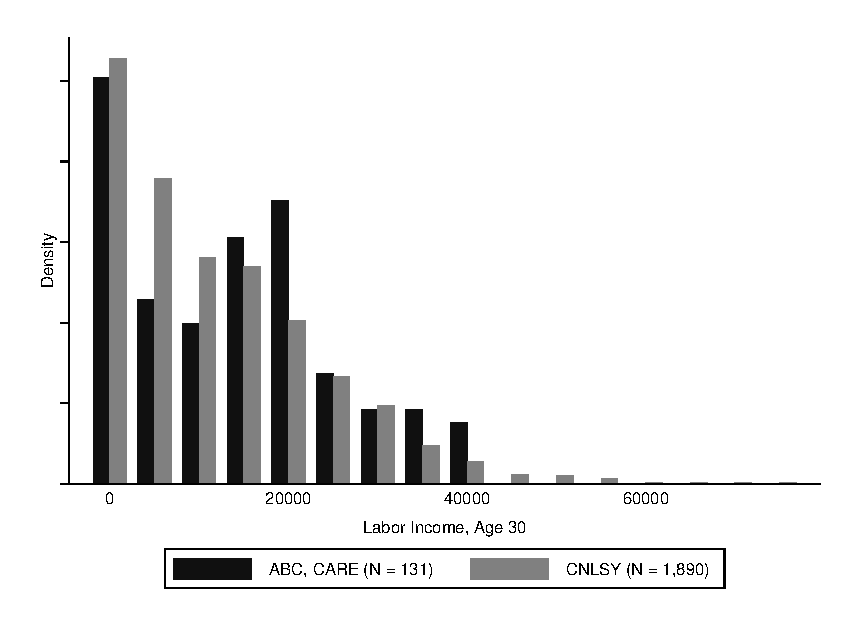
\includegraphics[width=\textwidth]{AppOutput/Methodology/support_inc21.eps}
	\end{subfigure}
	
	\begin{subfigure}[h]{0.9\textwidth}
	\centering
	\caption{Income at Age 30} \label{fig:support_inc30}
	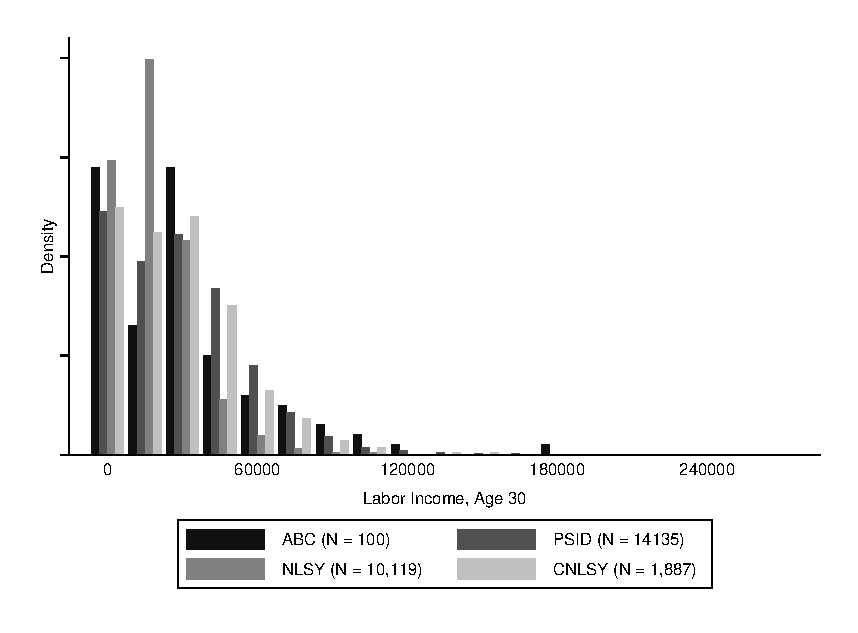
\includegraphics[width=\textwidth]{AppOutput/Methodology/support_inc30.eps}
	\end{subfigure}
\end{figure}




\begin{figure}[H]
	\ContinuedFloat
	\begin{subfigure}[h]{0.9\textwidth}
	\centering
	\caption{Subject's Years of Education} \label{fig:support_educ}
	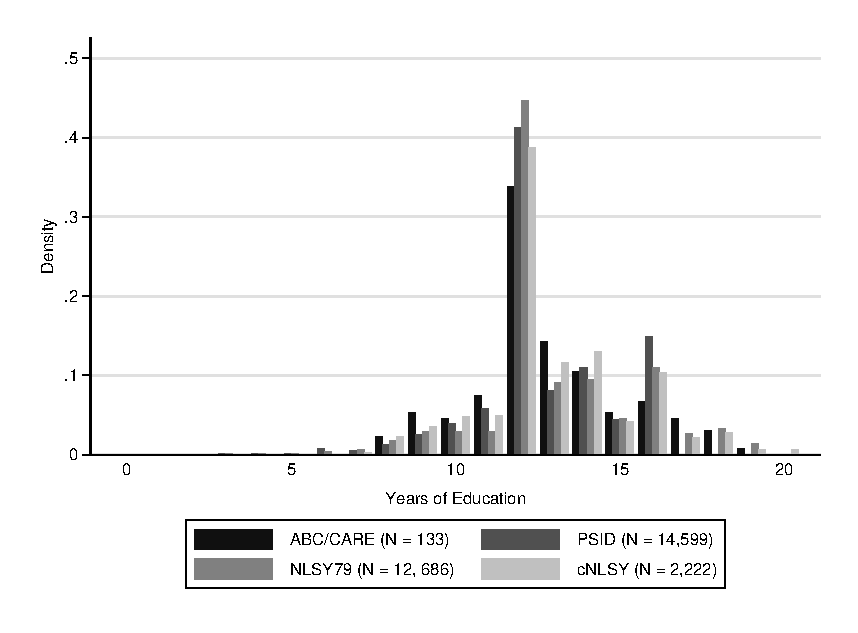
\includegraphics[width=\textwidth]{AppOutput/Methodology/support_educ.eps}
	\end{subfigure}
	
	\begin{subfigure}[h]{0.9\textwidth}
	\centering
	\caption{Mother's Years of Education} \label{fig:support_meduc}
	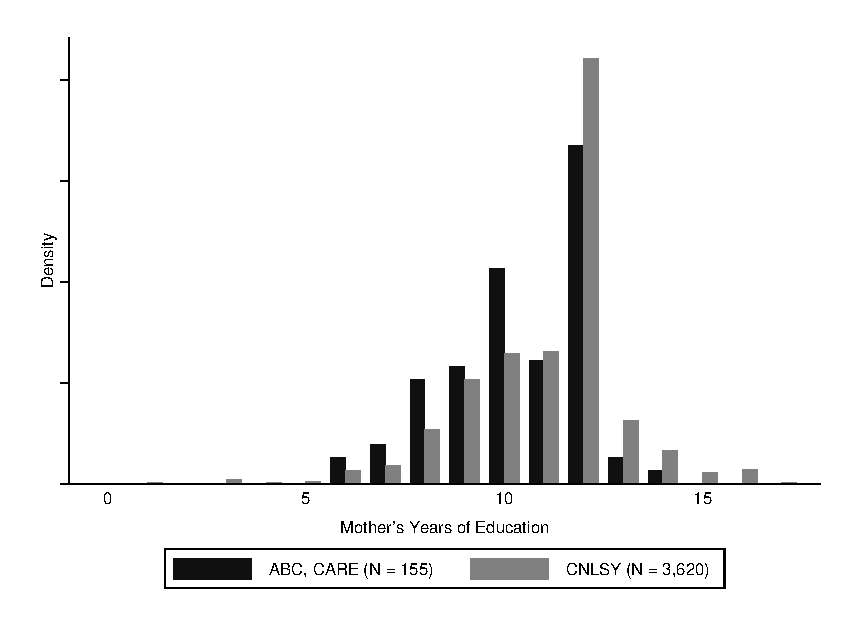
\includegraphics[width=\textwidth]{AppOutput/Methodology/support_momed.eps}
	\end{subfigure}
	
\end{figure}
	
\begin{figure}[H]
	\ContinuedFloat
	\begin{subfigure}[h]{0.9\textwidth}
	\centering
	\caption{Average PIAT Math Scores, Ages 5--7} \label{fig:support_math}
	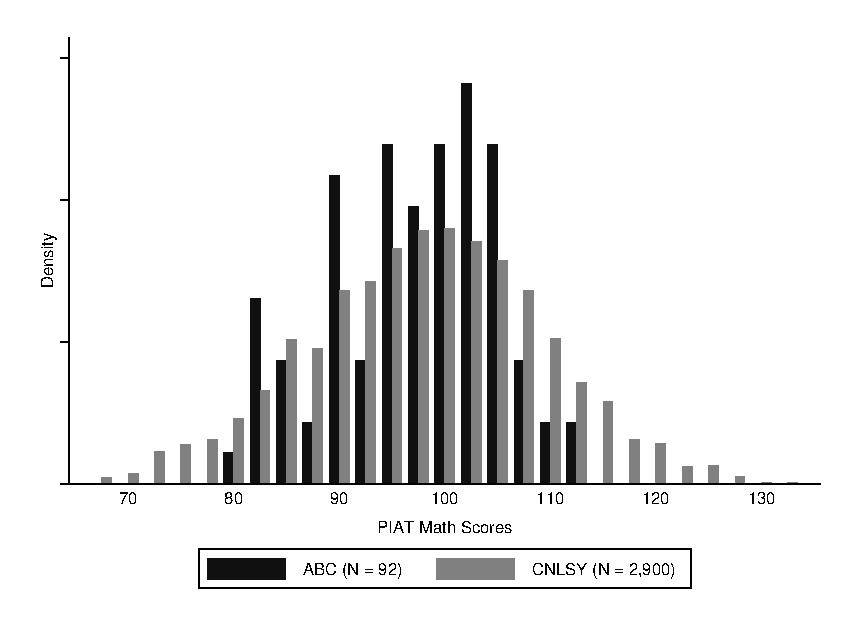
\includegraphics[width=\textwidth]{AppOutput/Methodology/support_math.eps}
	\end{subfigure}
	
	\begin{subfigure}[h]{0.9\textwidth}
	\centering
	\caption{Body Mass Index, Age 34} \label{fig:support_bmi}
	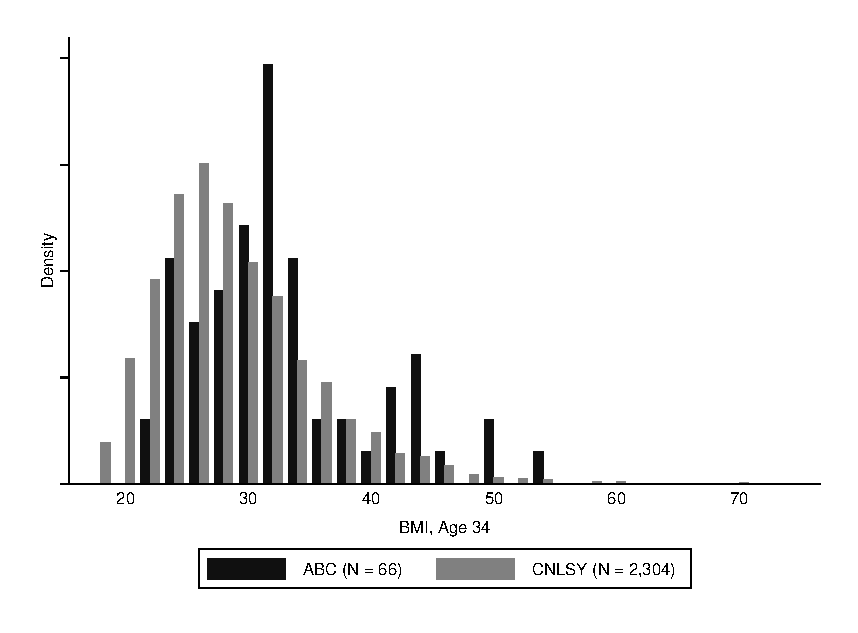
\includegraphics[width=\textwidth]{AppOutput/Methodology/support_bmi.eps}
	\end{subfigure}
	
	\floatfoot{
	\footnotesize
	\noindent Note: These graphs display the support of ABC, PSID, NLSY, and CNLSY
	for variables we use to project future earnings. PIAT math
	scores are averaged over ages 5--7.
	}
\end{figure}

\noindent Both labor and public-transfer income are interpolated using the exact same methodology, so we restrict
our description to interpolating labor income. We employ the CNLSY dataset to model labor
income at each age from 22 to 29. We use ordinary least squares and regress the labor income of
CNLSY subjects on background characteristics and early adult outcomes. Variables for background
characteristics consist of an indicator for being  black, mother's education, and sex. Variables
used to interpolate early adult outcomes consist of labor income at ages 21 and 30, years of education at age 30, average
PIAT math scores from ages 5 to 10, and BMI at age 34. We estimate the model on 1,000 bootstrap
resamples of the CNLSY to obtain a measure of prediction error, and denote the vectors of coefficients
\emph{for the outcome variables} by $\beta_{a,s}$, where $a \in \{22, 23, \dots, 29\}$ denotes age, and
$s \in \{1,2,\dots, 1,000\}$ indexes the bootstrap samples. \\

\noindent The outcome variables we use as independent variables to fit the model to the CNLSY data are also
observed in the ABC/CARE data, and we are able to calculate the treatment effects on each of these outcomes
using the procedures described in Appendix \ref{app:method_fullobs} and Appendix \ref{app:method_partialobs}. We
obtain these estimates for 1,000 bootstrap resamples of the ABC/CARE data, and denote the vectors of
coefficients by $\gamma_r$, where $r \in \{1,2,\dots,1,000\}$ indexes the bootstrap samples. \\

\noindent To interpolate the treatment effect on subject labor income at age $a$, we take the dot product
of $\beta_{a, s}$ and $\gamma_r$ for all $s,r$ pairs, resulting in 1,000,000 scalars. We reintroduce
prediction error by first randomly drawing residuals from our fitted model on the auxiliary data and assigning
them to the ABC/CARE subjects. We then take the mean difference of these residuals across treatment and control
groups, and add it to the previously described scalar. We do this for all 1,000,000 scalars. These scalars form the empirical
bootstrap distribution of the treatment effect. Note that
we bypass the estimation of the subjects' actual incomes, for which we are unable to obtain an
unbiased estimate. Instead, we directly obtain an unbiased estimate of the treatment effect. This
method implies that the impacts of the treatment on adult labor income can be expressed through
the observed early-adult outcomes. In this case, the observed early-adult outcomes are labor income at ages 21 and
30, years of education at age 30, average PIAT math scores from ages 5 to 10, and BMI at age 34. Since $\gamma_r$ has
been adjusted to address selection into treatment and attrition in the ABC/CARE data, the bootstrap distribution
is devoid of selection and attrition issues. In addition, the bootstrap distribution captures
the error stemming from the ABC/CARE dataset and the prediction error of the model fitted to the CNLSY dataset.
We take the mean of the empirical bootstrap distribution as our point estimate, and the standard deviation
of the distribution as the standard error. Again, we carry out this procedure for the
pooled, male, and female samples. \\

\noindent To extrapolate labor income, we employ the NLSY and PSID datasets. We execute the same estimation
strategy as above, but with a reduced set of control variables in order to limit the number
of dropped cases. Specifically, the set of background variables we control for include an indicator for
being black and gender of the subject. As the NLSY and PSID are not as rich as the CNLSY, we also
restrict our outcome variables to years of education at age 30 and subject labor income at age 30. \\
% Similar to the CNLSY, we restrict the PSID to individuals born between 1945 and 1980. As the PSID
% extends until 2013, this means we are using the most recent subsample of individuals aged 30 to 67.
% We do not impose a restriction on birth year on the NLSY as all respondents are aged between 47 and 55
% at the time of the last interview (conducted in 2012). For both the PSID and NLSY, subjects with labor
% income exceeding \$300,000 (USD 2014) are again excluded. Like the CNLSY, because of the biennial
% nature of the PSID and NLSY, we apply a linear interpolation to both data sets.

\noindent We estimate the vectors $\beta_{a, s}$ for $a \in \{31, 32, \dots, 67\}$ and $\gamma_r$, where
$s,r \in \{1,2,\dots,1,000\}$ index the bootstrap samples, and take the dot product of every pair of
$\beta_{a,s}$ and $\gamma_r$ vectors to obtain the empirical bootstrap distribution of the treatment
effect on labor income past age 30. We take the mean of the distribution to be the point estimate,
and the standard deviation of the distribution to be the standard error. \\

%The same procedure is carried out to interpolate and extrapolate transfer income, where we instead
%utilize transfer income as the dependent variable in the regressions on our auxiliary datasets.

\noindent The same procedure is carried out to interpolate public-transfer income, where we instead utilize public-transfer
income as the dependent variable in the regressions on our auxiliary datasets. In the case of
extrapolating public-transfer income from welfare, unemployment benefits, AFDC, and food stamps, we also apply
the same methodology as for labor income. However, in the case of disability insurance, social
security, and supplemental security income, we apply an alternative approach. For these variables, we estimate
the probability each ABC/CARE individual claims each of those benefits at ages 31--67, and multiply those
probabilities by the average annual claims of each type of public transfer reported by the Social
Security Administration in 2014. See Appendix \ref{section:FAM_ABC_impute}
for an explanation of how we estimate these probabilities. For each age, we sum across our estimates of
each type of public transfer received to obtain the total public-transfer income of both ABC/CARE subjects. \\


\paragraph{Health Costs}

\noindent We predict health care costs from age 30 up to age 79, and criminal costs from birth
up to age 50. We then evaluate the predicted outcomes as if observed, and estimate the
treatment effect on those data.\\

\noindent As health outcomes are simulated using a set of variables exhibiting a high rate of attrition, the
predicted health outcomes exhibit an equal rate of attrition. We therefore employ the method described
in Appendix \ref{app:method_partialobs} to estimate the treatment effect on health care costs at
every age from 30 through 79, conditional on survival up to each age. \\

\paragraph{Crime Costs}

\noindent In the case of crime costs, we are able to predict costs for more than 100 individuals in the
sample. We therefore utilize the method described in Appendix~\ref{app:method_fullobs}
to estimate the treatment effect on the cost of criminal activity at every age from birth until age 50. \\

\subsection{Internal Rate of Return}
\label{app:method_irr}

\noindent To estimate the internal rate of return, we must solve for $\rho$ in the equation below,

\begin{align}
\sum_{t=0}^T \frac{ \mathbb{E} (B_t - C_t)}{(1+\rho)^t} = 0,
\end{align}

\noindent where we let $T = 79$, define $B_t$ and $C_t$ to be the total benefits and costs of the program at time $t$, and define $\mathbb{E}(.)$ to be the sample mean. That is, we estimate the internal rate of return for the \textit{average subject} of ABC/CARE. \\

\noindent All outcomes of the parents and subjects that we observe as having been affected by the program are treated as benefits. For this to make sense, we reverse the sign of the monetized effect of the program on specific outcomes. Costs of ABC/CARE consist only of the initial program costs from ages 0 to 5. Table \ref{table:bc_comp} provides a full list of the benefits and costs of ABC. \\

\noindent We take the sum of the treatment effects on each component of the benefits to be the total benefit, $B_t$, of the ABC/CARE program (see Appendix \ref{app:method_identify} on how we estimate these treatment effects). This includes parental income, subject labor income, and QALYs (quality-adjusted life years). Treatment effects on costs borne by the subject or society have their signs reversed and are included as benefits. We do this for subject public-transfer income, education costs, crime costs, control substitution costs, and health costs. To account for deadweight loss, we impose a marginal welfare cost of 50\% by multiplying public costs by a factor of $1.5$.\footnote{There is no clear consensus on the marginal welfare cost of tax revenue. However, most researchers estimate the welfare cost per tax dollar to be between \$0.30 and \$0.50. See \citet{Feldstein_1999_REStat}, \citet{Heckman_Smith_1998_evaluating}, and \citet{Browning_1987_AER}.} Public costs include education costs up until age 17, jail costs, justice system costs, Medicare costs, Medicaid costs, disability insurance claims, social security claims, and supplemental security income. \\

\noindent Having constructed our cash flow, $\mathbb{E} (B_t - C_t)$, solving for $\rho$
reduces to an algebraic exercise. \\

\noindent As described in Appendix \ref{app:method_identify}, we estimate the treatment effect on each
component of the benefits and costs at time $t$ for the pooled, male, and
female samples. We do this for 1,000 bootstrap resamples of the original ABC/CARE data.
In the case of health costs and subject income, for which we employ auxiliary datasets to
estimate the treatment effects, we also obtain 1,000 bootstrap estimates from the auxiliary data
for every ABC/CARE bootstrap resample, resulting in a total of 1,000,000 estimates.
By reusing each bootstrap estimate of the treatment effect on outcomes that do not require any auxiliary data
set 1,000 times, we obtain a total of 1,000,000 estimates of the cash flow.
We estimate the internal rate of return on each of those cash flows.
This is how we form our empirical bootstrap distribution of the internal rate of return for the pooled, male, and female samples.
We take the mean of the distributions to be the point estimates, and we take the standard deviations
to be the standard errors. To construct the 80\% confidence intervals, we take the 10\textsuperscript{th}
and 90\textsuperscript{th} quantiles of each bootstrap distribution. \\

\noindent \textbf{[JJH: What is the basis for the 0.5 in public-transfer income? Why the 1.5?]} \\
\noindent \textbf{[JLG: basis is \citet{Browning_1987_AER,Heckman_Smith_1998_evaluating,Heckman_LaLonde_etal_1999_active,Feldstein_1999_REStat}, which is the basis for the Perry CBA as well.]}

% We let $T = 79$. In Appendix \ref{app:method_identify}
% we explain how we can estimate the summand of the numerator at every period $t$, which
% can be expressed as $\mathbf{E}(B_t) -  \mathbf{E}(C_t)$. Thus, solving for $\rho$
% reduces to an algebraic exercise.



% To construct our cash flow, we subtract the costs from benefits to create a single stream.
% We define `cost' to include only the program costs of ABC, and define
% `benefits' to include all treatment effects of the program. This includes
% the treatment effects on parent income, subject labor income, and QALY
% (quality adjusted life years).\footnote{QALYs are measured on a scale of 0 to 1, with 1 being a
% year of perfect health. We follow \textbf{[CITATION]} and value a QALY of 1 to be
% \$150,000, and a QALY of 0 to be \$0. The dollar value of that year relates linearly to the QALY.}
% Treatment effects on costs borne by the subject or society have their signs
% reversed and are included as benefits. We do this for subject transfer income,
% education costs, jail costs, justice system costs, victimization costs,
% control contamination costs, and medical costs. To account for deadweight loss, we
% impose a marginal welfare cost of 50\% by multiplying public costs by a factor of
% $1.5$.\footnote{There is no clear consensus on the marginal welfare cost of tax revenue. However,
% most researchers estimate the welfare cost per tax dollar is between \$0.30--0.50. See
% \citet{feldstein1999tax, heckman1998evaluating, browning1987marginal}.} This
% includes education cost up until age 17, jail costs, justice system costs, Medicare costs,
% and Medicaid costs. For the same reason, we multiply transfer income by a factor of 0.5.

% For each period $t \in \{1, 2, \dots, 79\}$, we sum our estimates of the benefits, and
% subtract our estimates of the costs from that sum. This provides us an estimate of
% $\mathbf{E}(B_t) -  \mathbf{E}(C_t) = \mathbf{E} (B_t - C_t)$. We then solve for
% $\rho$ using numerical analysis.

% In your methodlogy you describe costs and benefits differnetly....
% To construct our cash flow, we sum the costs and benefits from the program into a single stream.
% We define `cost' to include only the cost of implementing ABC. On the other hand,
% we broadly define `benefits' to include all treatment effects of the program. This includes
% the treatment effects on parent income, subject labor income, and QALY
% (quality adjusted life years).\footnote{QALYs are measured on a scale of 0 to 1, with 1 being a
% year of perfect health. We follow \textbf{[CITATION]} and value a QALY of 1 to be
% \$150,000, and a QALY of 0 to be \$0. The dollar value of that year relates linearly to the QALY.}
% Treatment effects on outcomes generally considered to be costs have their signs reversed in
% order to convert them into benefits. We do this for subject transfer income,
% education costs, jail costs, justice system costs, victimization costs,
% control contamination costs, and medical costs. To account for deadweight loss, we
% impose a marginal welfare cost of 50\% by multiplying public costs by a factor of
% $1.5$.\footnote{There is no clear consensus on the marginal welfare cost of tax revenue. However,
% most researchers estimate the welfare cost per tax dollar is between \$0.30--0.50. See
% \citet{feldstein1999tax, heckman1998evaluating, browning1987marginal}.} This
% includes education cost up until age 17, jail costs, justice system costs, Medicare costs,
% and Medicaid costs. For the same reason, we multiply transfer income by a factor of 0.5.


\subsection{Computing the Benefit/cost Ratio}
\label{app:method_cbratio}

\noindent The benefit/cost ratio can be expressed as,

\begin{align}
\mathbb{E} \left( \frac{ \sum_{t=0}^T B_t}{\sum_{t=0}^T C_t} \right),
\end{align}

\noindent where we let $T = 79$, define $B_t$ and $C_t$ to be the total benefits and costs of the
program at time $t$, and define $\mathbb{E}(.)$ to be the sample mean. See Table \ref{table:bc_comp} for a detailed list of the components
to the benefits and costs of ABC/CARE . We take the sum of the treatment effects on each component
of the benefits to be the total benefits of the ABC/CARE programs (see Appendix~\ref{app:method_identify} on how we estimate these treatment effects). \\

\noindent To account for deadweight loss, we assume a marginal welfare cost of 50\% by multiplying
public costs components by a factor of $1.5$. For the same reason, we multiply public-transfer
income by a factor of 0.5 \textbf{[JJH: Why? What principle?]}\textbf{[JLG: See previous comment. We base this on Perry CBA.]}. We discount each component of the benefits and costs
by 3\% every year to obtain their net present value at birth. We then sum up the discounted
components of the benefits and find the ratio with the discounted costs. \\

\noindent As described in Appendix \ref{app:method_identify}, we estimate the treatment effect on each
component of the benefits and costs at time $t$ for the pooled, male, and
female samples. We do this for 1,000 bootstrap resamples of the original ABC/CARE data.
In the case of health costs and subject income, for which we employ auxiliary datasets to
estimate the treatment effects, we also obtain 1,000 bootstrap estimates from the auxiliary data
for every ABC/CARE bootstrap resample, resulting in a total of 1,000,000 estimates.
By reusing each bootstrap estimate of the treatment effect on outcomes that do not require any auxiliary data
set 1,000 times, we obtain a total of 1,000,000 estimates of the costs stream and benefits stream.
We estimate the benefit/cost ratio for each of those streams.
This is how we form our empirical bootstrap distribution of the benefit/cost ratio for the pooled, male, and female samples.
We take the mean of the distributions to be the point estimates, and we take the standard deviations
to be the standard errors. To construct the 80\% confidence intervals, we take the 10\textsuperscript{th}
and 90\textsuperscript{th} quantiles of each bootstrap distribution.

\begin{table}[H]
\begin{threeparttable}
\caption{Components of Benefits and Costs}
\label{table:bc_comp}
\centering
\begin{tabular}{l c c}
\toprule			
Variable & Sign Reversed	& Welfare Cost \\
	&		& Factor \\
\midrule
\textbf{Benefits} 	\\			
\quad Parent Income			& \\
\quad Subject QALY			& \\
\quad Subject Labor Income	& \\
\quad Subject Public-transfer Income	& $\checkmark$	& 0.5 \\
\quad Medicare Costs			& $\checkmark$	& 1.5 \\
\quad Medicaid Costs			& $\checkmark$	& 1.5 \\
\quad Out-of-pocket Medical Costs	& $\checkmark$ \\
\quad Miscellaneous Medical Costs	& $\checkmark$ \\
\quad Disability Insurance Claim	& $\checkmark$	&	1.5 \\
\quad Social Security Claim	& $\checkmark$	&	1.5 \\
\quad Supplemental Security Claim	& $\checkmark$	&	1.5 \\
\quad Control Substitution Costs	& $\checkmark$	& \\
\quad Education Costs			& $\checkmark$	& 1.5* \\
\quad Justice System Costs	& $\checkmark$	& 1.5 \\
\quad Prison Costs			& $\checkmark$	& 1.5 \\
\quad Victimization Costs		& $\checkmark$	& \\
\textbf{Costs} 	\\			
\quad Program Costs			& \\
\bottomrule			
\end{tabular}
\begin{tablenotes}
\footnotesize
\item Note: The table lists the components of the costs and benefits of ABC/CARE.
In order for some components to be categorized as benefits, we reversed the sign
of the treatment effect. *Only education costs up until age 18 are multiplied by 1.5 to account for welfare costs. This factor is drawn from \citet{Heckman_Moon_etal_2010_RateofReturn}.
\end{tablenotes}
\end{threeparttable}
\end{table}


